\subsection{Gradients for 1D regression problem}
\label{app:toy_example_gradients}
In this section, we analytically derive the gradient descent (GD) updates for the latent weight the 1D toy regression example of section \ref{sec:oscillations}.
% derive analytical expressions for the gradient descent updates of the latent weight from the 1D toy regression example of section \ref{sec:oscillations}.
We compare the gradient from the vanilla STE with other methods from the literature (cf. section \ref{sec:backgroundrelated}) and our proposed oscillation dampening solution (cf. section \ref{sec:oscillations_dampening}). We define $\bar{w}$ as the boundary between the two quantization levels closest to the optimal value $w_*$, such that $\bar{w}= (\up{w}+\down{w})/2$, where $\up{w}=q(w_*+\frac{s}{2})$  and $\down{w}=q(w_*-\frac{s}{2})$.

The gradient of the mean-squared loss from equation \eqref{eq:toy_regression_optim} w.r.t. to the weight is given by: 
%
\begin{align} 
    \frac{\partial \tlossb(w)}{\partial w}& =\sigma^2 \left(q(w) - w_* \right)  \frac{\partial q(w)}{\partial w }, \\
    &= \begin{cases}
    \sigma^2 \left(\up{w} - w_*\right)\frac{\partial q(w)}{\partial w } , & \text{if }w \geq \bar{w} \\
    \sigma^2 \left(\down{w} - w_* \right) \frac{\partial q(w)}{\partial w },& \text{if } w < \bar{w}\\
    \end{cases} 
    \label{eq:regression_grad_quant}
\end{align}
%

Assuming $\sigma=1$, a learning rate of $\eta$, and that no clipping takes place we write the GD update rules for subset of methods discussed in section \ref{sec:backgroundrelated}. For the PSG \citep{PBGS}, the update rule includes an arbitrarily small constant, $\epsilon>0$, while EWGS  \citep{EWGS} introduce a $\delta \geq 0$ scaling factor. 

\begin{center}
\begin{tabular}{ l | l } 
STE &  
$w_{t+1} = 
    \begin{cases}
    w_t - \eta  \left(\up{w} - w_* \right),   & \text{if }w \geq \bar{w}\\ 
    w_t - \eta  \left(\down{w} - w_* \right), & \text{if } w < \bar{w}\\
    \end{cases}$\\
    \\[-0.5em]
PSG  \citep{PBGS} & $ w_{t+1} = \begin{cases}
    w_t - \eta  \left(\up{w} - w_* \right)   \left(\up{w} -w + \epsilon\right),   & \text{if }w \geq \bar{w}\\
    w_t - \eta  \left(\down{w} - w_*\right) \left(w - \down{w}+ \epsilon\right),  & \text{if } w < \bar{w}\\
    \end{cases}$ \\
    \\[-0.5em]
  EWGS  \citep{EWGS} & $ w_{t+1} = \begin{cases}
    w_t - \eta  \left(\up{w} - w_* \right) \left(1+ \delta \left( w -\up{w}\right)\right), & \text{if }w \geq \bar{w}\\
    w_t - \eta  \left(\down{w} - w_*\right) \left(1- \delta \left(w - \down{w}\right)\right), & \text{if } w < \bar{w}\\
    \end{cases}$ \\
    \\[-0.5em]
  Dampening (sec. \ref{sec:oscillations_dampening}) & $ w_{t+1} = \begin{cases}
    w_t - \eta  \left(\up{w} - w_* + 2\lambda \left(w - \up{w}\right)\right), & \text{if }w \geq \bar{w}\\
    w_t - \eta  \left(\down{w} - w_* + 2\lambda \left(w - \down{w}\right)\right), & \text{if } w < \bar{w} \\
     \end{cases}$\\
       \\[-0.5em]
%   Cosine & $ w = \begin{cases}
%     w - \alpha \cdot (w^* - w^+ + \lambda \pi \theta sin(\pi \theta w)) & \text{if } w > (w^+ + w^- / 2)\\
%     w - \alpha \cdot (w^* - w^-+ \lambda \pi \theta sin(\pi \theta w)) & \text{if } w < (w^+ + w^- / 2) \\
%      \end{cases}$
\end{tabular}
\end{center}

If we look at the equations for PSG and EWGS more carefully, we see that they introduce an \textit{always positive} scaling term to the STE gradient (assuming sufficiently small $\delta$) . Therefore, these methods can only change the magnitude of the update and not its direction, meaning they cannot stop oscillations from happening. Because the methods apply a  scaling to the STE gradient, we call them \textit{multiplicative} variations in section \ref{sec:related_work}. 

On the other hand, our dampening method adds an extra term to the gradient, which is of opposite sign to the STE gradient. Thus, this \textit{additive} variation of the STE can indeed prevent oscillations by changing the direction of the gradient.

% We observe that PSG and EWGS apply a \textit{positive }scaling factor to the STE gradient,

% why we call them \textit{multiplicative} variations in section \ref{sec:related_work}. 



% \subsection{PSG and EWGS}
% \label{app:psg_ewgs}
% We can see that PSG and EWGS are the same method, up to a different parametrization. If we divide the gradient term in PSG by $\epsilon$, and rewrite $\alpha = \alpha / \epsilon$ the update rules are exactly the same. However, this is not completely in the spirit of both papers. The PSG paper suggests having only a very small $\epsilon = 1e-4$ for stability purposes, which would correspond to a very large $\delta$ in PSG and a strong effect on the scaling of the learning rate that we are unsure of how the authors correct for. In spirit, PSG seems to suggest having a very large $\delta$ in the EWGS setting, whereas EWGS itself uses a very small $\delta$, seemingly contradicting each other. 

\subsection{Relation of the distance and frequency}
\label{app:relation_distance_frequency}

In toy example of section \ref{sec:oscillations}, we explained how the frequency of the oscillations depends linearly on distance of the optimal weight value $w_*$ from its closest quantization level $q(w_*)$. We can, thus, define the oscillation frequency as:
\begin{equation}
    f = \frac{|q(w_*) - w_*|}{s},
    \label{eq:toy_example_freq}
\end{equation}
where $s$ is the quantization scaling factor or size of the quantization bin. The frequency depends linearly on the distance $d= |q(w_*) - w_*|$ due to the squared error loss. In figure \ref{fig:oscillation_frequency}, we demonstrate this dependency experimentally by varying the distance $d$ and observing the effect on the oscillation frequency.

\begin{figure*}[h]  
\centering
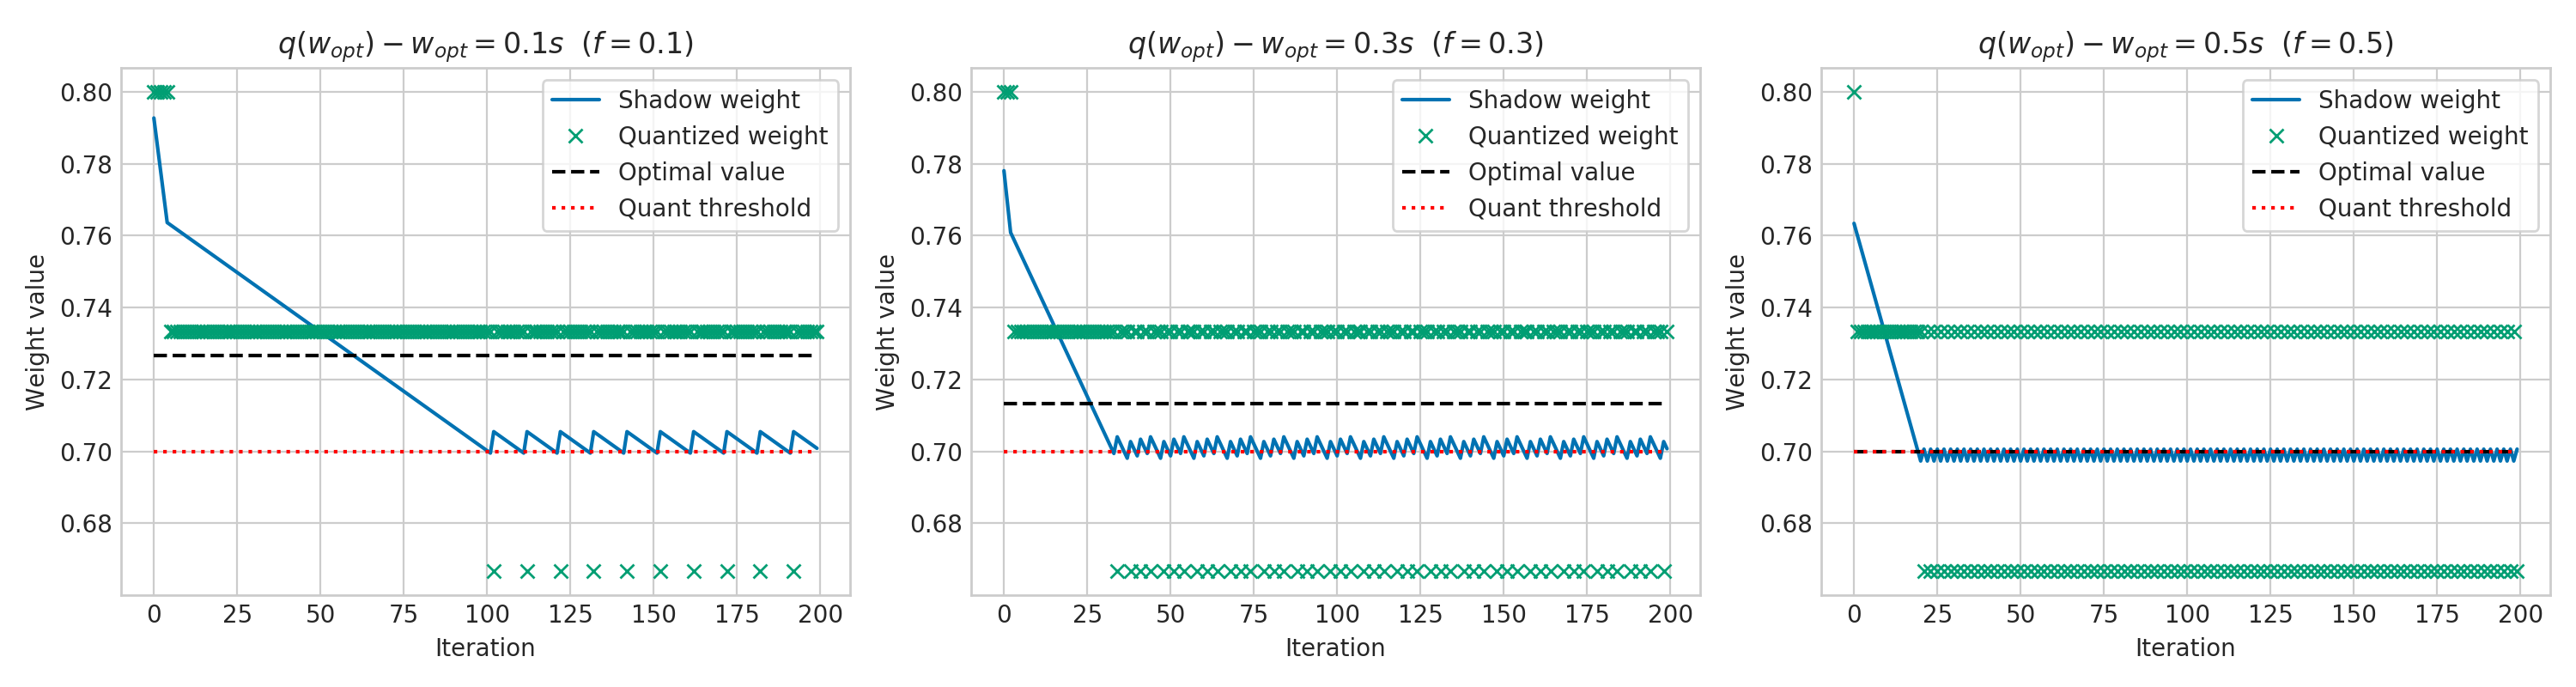
\includegraphics[width=0.9\textwidth]{figures/toy_example_frequency.png}
\caption{Oscillation  of single weight in toy-regression problem for optimal values. The distance between the closest quantization point and the optimal value directly corresponds to the oscillation frequency.}
\label{fig:oscillation_frequency}
\end{figure*}

% In figure \ref{fig:oscillation_frequency} we show the relation between the oscillation frequency and the distance of the optimal weight value. We can see that the frequency of the oscillation is linearly depending on the distance of the optimal value compared to the closest quantization point. We also reasoned about this in section \ref{sec:oscillations}. We thus define the oscillation frequency for our toy example as:
% \begin{equation}
%     f = \frac{|q(w_*) - w_*|}{s},
% \end{equation}
% where $s$ is the quantization scaling factor or size of the quantization bin. The frequency depends linearly to the $|q(w_*) - w_*|$ because of the squared error loss.

% This is because the mean square d error in our optimization is based on the distance to the quantized point. It is easy to see that on such a toy example the gradient is 
% \begin{equation}
%     \frac{\partial}{\partial w} \frac{1}{2} (q(w) - w_*)^2 = q(w) - w_*
% \end{equation}
% and thus its magnitude linearly depend on the distance to the optimal value. 

\subsection{Different learning rates and multiplicative regularization methods}
\label{app:learning_rates_oscillation}
\begin{figure*}[ht]  
\centering
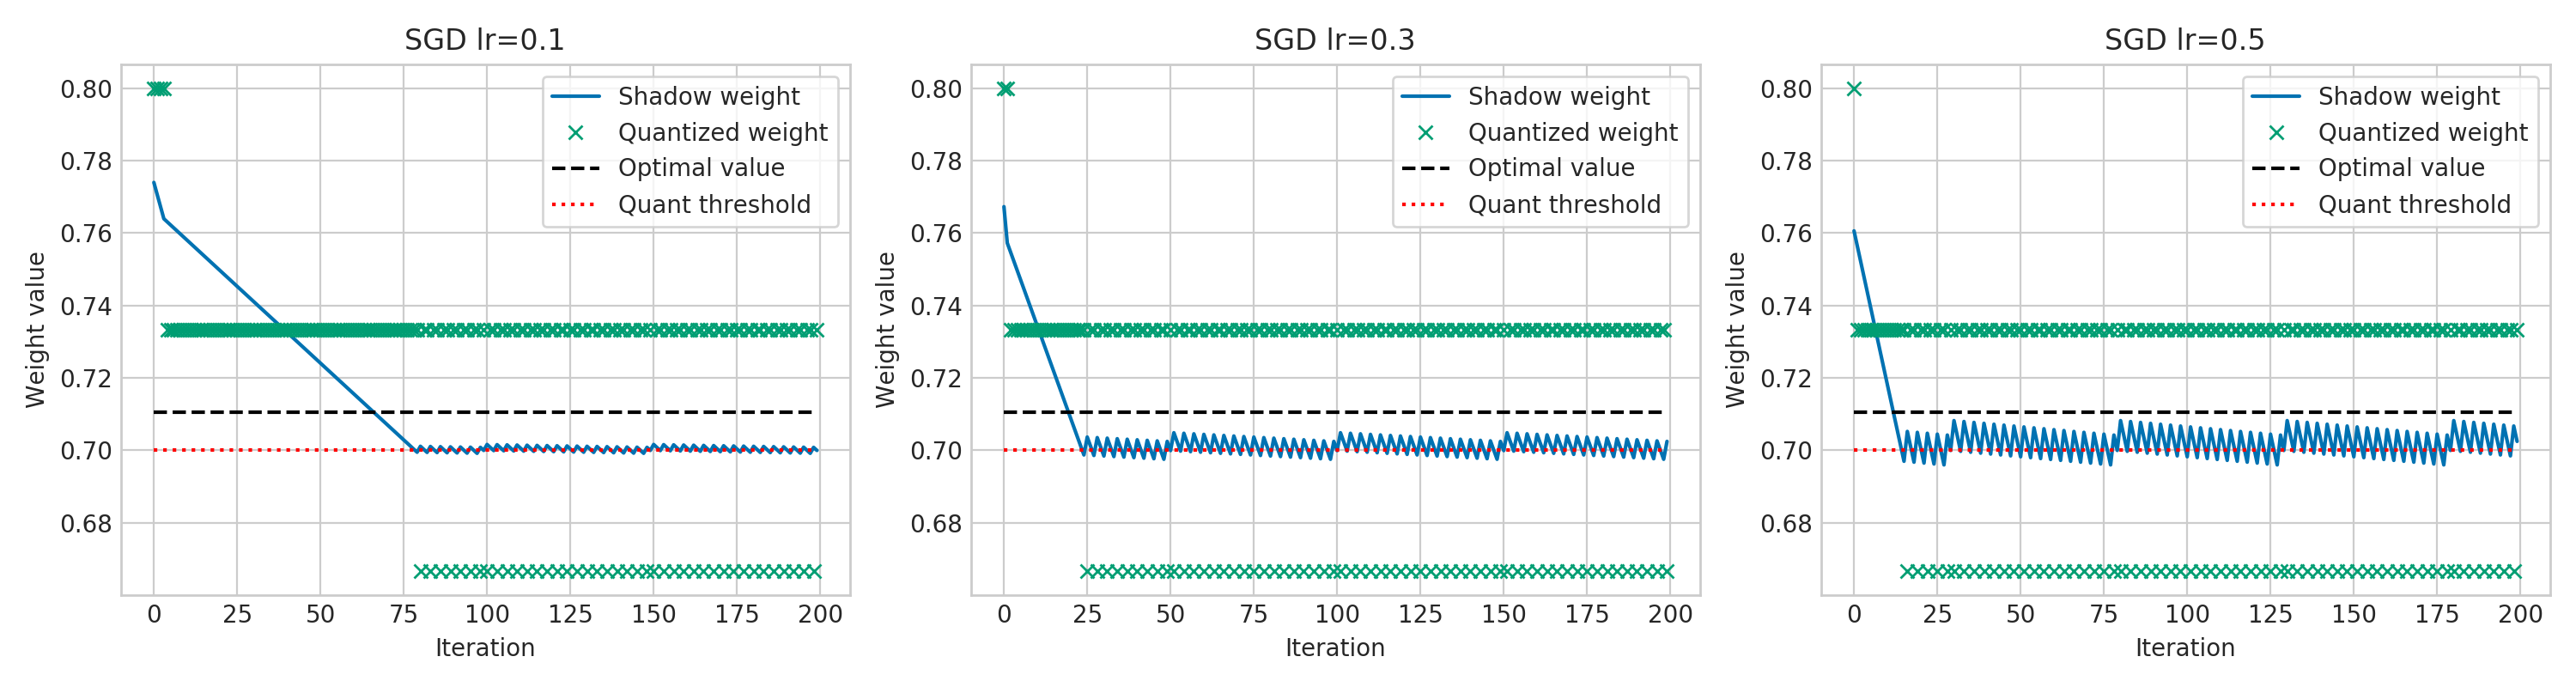
\includegraphics[width=0.9\textwidth]{figures/toy_example_lrs.png}
\caption{Oscillation  of single weight in toy-regression problem for various learning rates (with STE).}
\label{fig:oscillation_lrs}
\end{figure*}


In figure \ref{fig:oscillation_lrs}, we plot the latent weight in our toy regression example for different learning rates assuming STE gradients. We can see that the change in learning rate only influences the amplitude of the oscillations and not the oscillation frequency. 

% As we can see from figure \ref{fig:oscillation_lrs}, a change in learning rate only influences the amplitude of oscillations but the oscillation frequency is unaffected.
This is also apparent from equation \eqref{eq:toy_example_freq}, which shows that the frequency is independent of the learning rate. Theoretically, this suggests that \textit{multiplicative} variations of the STE, such as EWGS and PSG, cannot prevent oscillations from occurring.
% This also means that the multiplicative methods from the related work section \ref{sec:backgroundrelated}, such as EWGS and PSG, do not entirely, in theory, prevent the oscillations from occurring.
Assuming a sufficiently small learning rate, weights will in the limit still converge to the decision threshold and start oscillating. While oscillating, the distance of the oscillating weight from its two closest quantization levels is roughly constant and equal to $s/2$.
This means that close to the decision threshold the weight update rules for PSG and EWSG become:
\begin{center}
\begin{tabular}{ l | l } 
PSG  \citep{PBGS} & $ w_{t+1} = \begin{cases}
     w_t - \eta  \left(\frac{s}{2}+ \epsilon\right) \left(\up{w} - w_*\right)  ,   & \text{if }w \geq \bar{w}\\
    w_t - \eta \left(\frac{s}{2} + \epsilon\right)  \left(\down{w}- w_* \right) ,  & \text{if } w < \bar{w}\\
    \end{cases}$ \\
    \\[-0.5em]
  EWGS  \citep{EWGS} & $ w_{t+1} = \begin{cases}
    w_t - \eta \left(1-  \frac{s\delta}{2}\right)  \left(\up{w} - w_*\right) , & \text{if }w \geq \bar{w}\\
    w_t - \eta \left(1-  \frac{s\delta}{2} \right)  \left(\down{w}-w_* \right) , & \text{if } w < \bar{w}\\
    \end{cases}$ \\
    \\[-0.5em]
\end{tabular}
\end{center}
Both methods now apply a constant and positive scaling to the gradient. Given that typically $s<1$, and that for EWGS $\delta<1$, the combined gradient scaling is $<1$ effectively reducing the learning rate and consequently the oscillation amplitude. This analysis is only valid if the oscillation amplitude is small, which is typical towards the end of training. However, in the earlier stages of training, where the weights move more freely, the dynamics of the oscillations might be more complicated, as the gradient or velocity of the weight depends on the distance from the closest quantization bin. 

% and less than 1 scaling factor to the gradient, leading to a slight dampening effect. Given that typically $$

% Although the PSG and EWGS methods do not prevent oscillations in our toy example, during a generally very noisy training process, both will make the representable grid-points stickier and ensure weights stay closer to the grid-points as opposed to the decision thresholds. 

% WWGS scales the gradient by a positive values less than 1, as 

% This is because the gradient in both cases is only multiplied by a positive value $\delta (-w + w^+) +1$ or $\delta (w + w^-) +1$ below the decision threshold. This means that in the limit the weight value will still converge to the decision threshold, and as long as the learning rate is sufficiently small stay there. There is a slight dampening effect of the learning rate modulation, but if the learning rate is small the weights will stay close to the decision threshold and the terms depending on $(-w + w^+) and (w + w^-)$ will be nearly constant. 

% Although the PSG and EWGS methods do not prevent oscillations in our toy example, during a generally very noisy training process, both will make the representable grid-points stickier and ensure weights stay closer to the grid-points as opposed to the decision thresholds. 


% \subsection{Stochastic Rounding}
% \label{app:stochastic_rounding}
% Another frequently used method for improving quantization-aware training is \textit{stochastic rounding} (SR). It also has a more elaborate cousin named relaxed-quantization \cite{louizos2018relaxed}. Stochastic rounding is a technique that can be dated back to 1950 as a solution to rounding errors in low-bit machines used for solving differential equations  \cite{1950forsythe}. In stochastic rounding, rather than rounding to the nearest grid-point, we instead round stochastically with a probability equal to the distance of the weight from its two closest grid-points.
% % rounding doesn't happen to the nearest value, but stochastically proportional to the distance of the rounded value to each grid-point.
% In our toy example setup we have:
% \begin{equation}
%     q_{\text{SR}}({w}) = \begin{cases}
%     \up{w} & \text{with probability } \l(\up{w} - w\r)/s  \\
%     \down{w} & \text{with probability } \l(w - \down{w}\r)/s\\
%     \end{cases}
% \end{equation}
% where $s$ is the size of the quantization bins or scaling factor from \eqref{eq:quantization_formulation}. We analyze how the STE compares to stochastic rounding in light of this toy example. As we can see in fig. \ref{somefig}, the weight value in stochastic rounding has the nice property it converges to $w^*$, and is susceptible to converge with decreasing learning rate. 

% The two methods are related. If we set $\down{w} = 0$, $\up{w}= 1$, $w_*=0.75$, in the STE case we see the period of the oscillations is $4$, and the sequence spends 3 iterations in $w^*$, and 1 iteration in $w^-$. We can see that the expectation over many iterations $\mathbb{E}_{w_t}\left[\round{w_t}_{SR}\right] = w^* = \mathbb{E}_{w_t}\left[\round{w_t}_{STE}\right]$. Ergo, in the limit the solution $\round{w}$ spends just as many iterations in $w^+$ in both the STE and stochastic rounding solutions.

% However, the two differ apparently on at least two accounts. Firstly, since the STE weight tends to the decision threshold in the limit, and the SR weight tends to the optimal value, any weight-decay will affect the two differently. It is unclear if this is significant, or beneficial to either, but it's a difference nonetheless. The second is that the introduced noise of SR is sampled in a Markovian fashion, whereas the STE oscillations introduce a stable cadence of roundings. This means that the introduced SR process is more noisy, as there is a higher chance it samples streaks of the same roundings when optimizing. It is possible it samples multiple improbable roundings in a row, which can affect optimization negatively.

% Because of the latter effect, we conjecture that the SR process adds more noise in optimization than the STE process. If this noise is unnecessary for regularization as described in \cite{polino2018distillation}, this can lead to reduced performance of the quantized model as described in \cite{krishnamoorthi}. We also verified this ourselves \ref{here}. 

% On the network level, we also see that a network trained with stochastic rounding has more un-decided weights than an STE trained model, despite the oscillations in convergence playing a role. This means that if we were to draw samples from the SR trained model, any of those will perform well. But as opposed to dropout where this process helps, in our setting we can't take the average over settings and have to make a single discrete choice from the space. \ref{some data on this from Yelysei} The best we can do in this case is round our weights to the nearest value, but we know from \cite{adaround} that this is not necessarily the best practice and can potentially lead to poor results in the aggregate. 

% \subsection{Weight distributions}
% \begin{figure}[t]
% \centering
% \vspace{-.0cm}
% 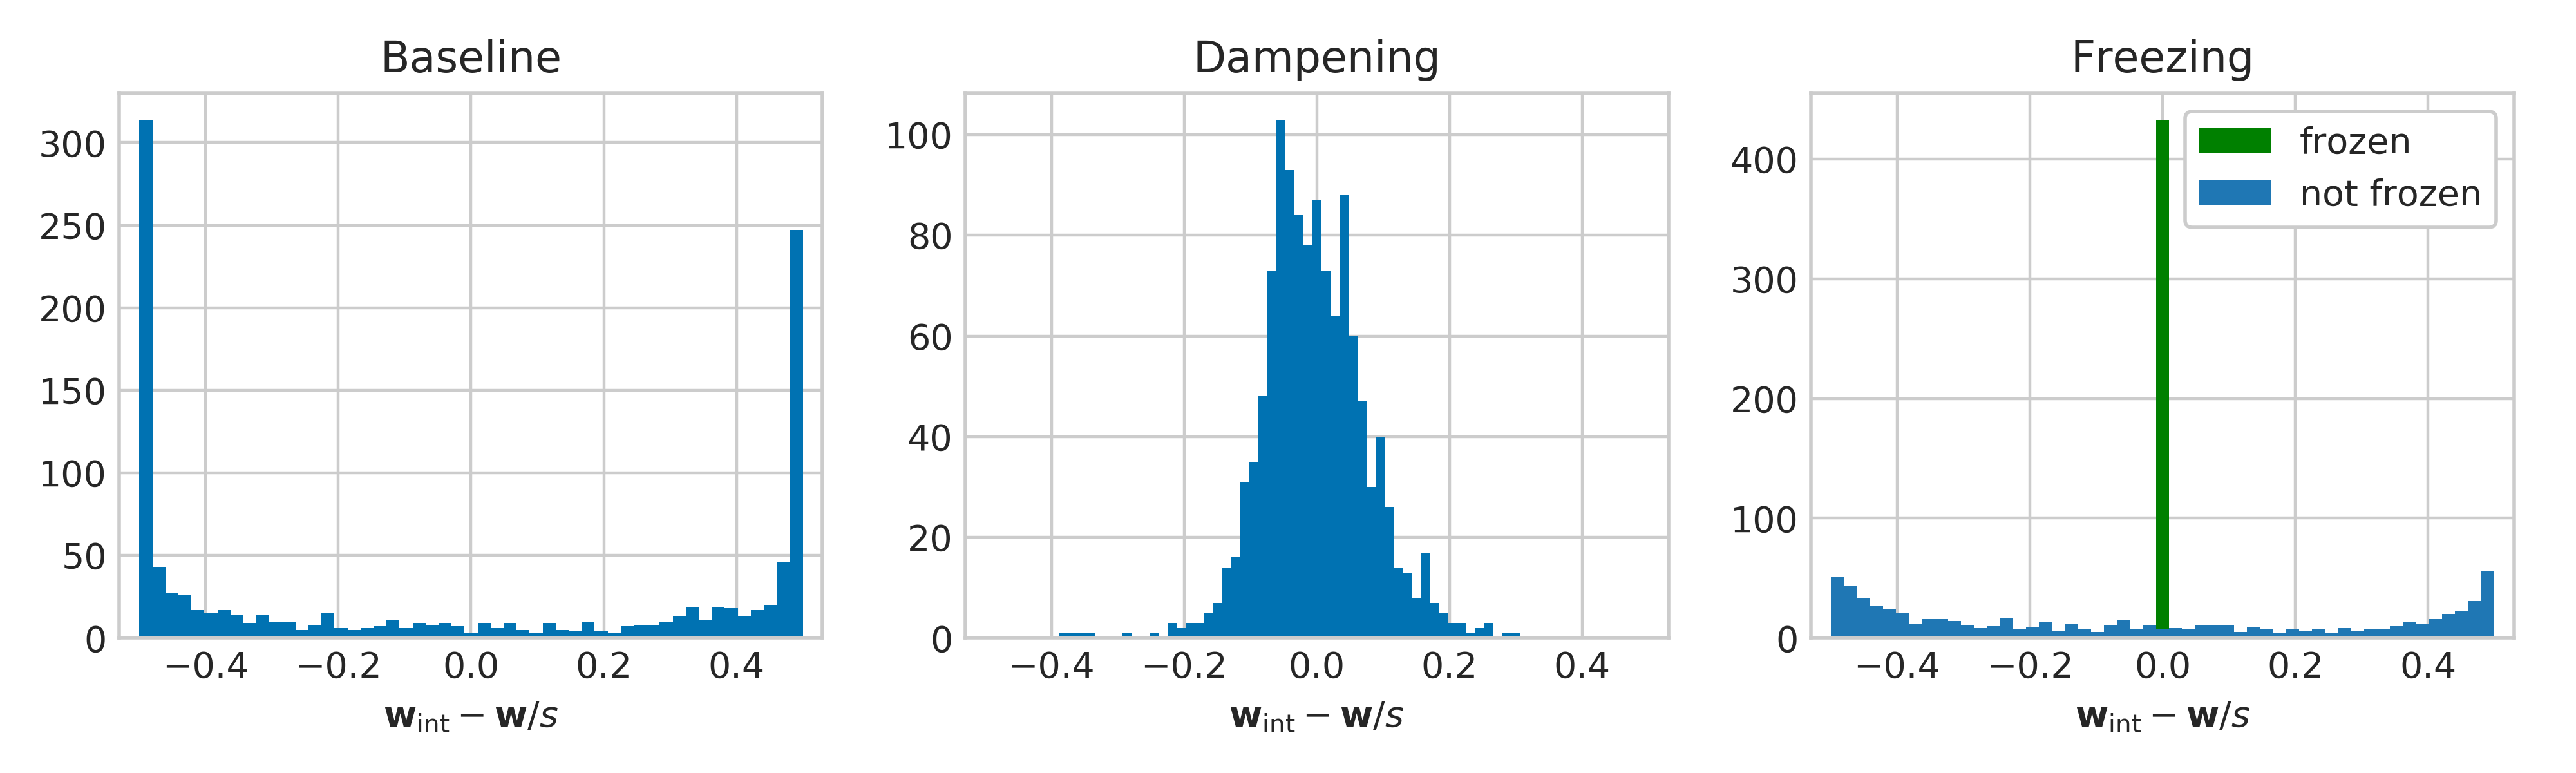
\includegraphics[width=.8\linewidth]{figures/mnv2_bin_dist_lsq_binReg_freeze.png} 
% \vspace{-.4cm}
% \caption{Depth-wise separable layer of third inverted residual block of \mnv{2} (conv.3.1): histogram of the distance of latent weight from their closest quantization grid-point for LSQ training (left), oscillation dampening (middle) and  iterative weight freezing (right).} 
% \vspace{-.2cm}
% \label{fig:bin_distribution_freezing_damp_appendix}
% \end{figure}

% In figure \ref{fig:mv2_bin_distribution} (right) we plotted the distance of the latent weight,  ($\vec{w}_{\INT} - \vec{w}/\ct{s}$), from their closest quantization grid-point during vanilla QAT for the depth-wise convolution (conv.3.1) of \mnv{2}. We saw that due to weight oscillating, the vast majority of the weights lie right at the boundary between quantization bins. In figure \ref{fig:bin_distribution_freezing_damp}, we now plot the same graph but
% after LSQ training with \textit{oscillation dampening} and \textit{iterative weight freezing} in place. We observe that dampening successfully pushes the distribution closer the quantization grid-point, while weight freezing fixes the majority of the weights to the quantization grid-point.


\subsection{The bias of the STE}
\label{app:biased_ste}
In the original paper on the straight-through estimator, \citet{bengio2013estimating} note that ``...\textit{(the STE) is clearly a biased estimator}''. Several authors, such as \citet{chmiel2022luq, fan2021extreme}, have repeated this statement and have argued that this \textit{bias} is a fundamental drawback of STE when applied to quantization, without defining what this actually means in the context of quantization-aware training.

% Several authors, such as \citet{chmiel2022luq, fan2021extreme}, have rolled with this explanation in their papers, talking about the bias as the chief drawback of the STE when applied to quantization, without defining what this actually means.

The bias of the STE in the original formulation occurs in a probabilistic setting. Let's assume we want to optimize a loss $\mathcal{L} = \mathbb{E}_{p(z|\theta)} \left[f(z)\right]$ where $z$ is latent parameter coming for a discrete distribution $p(z|\theta)$. To learn the parameter $\theta$ we need to calculate the derivative $\nabla_{\theta} \mathbb{E}_{p(z|\theta)} \left[f(z)\right]$. However, due to the discrete nature of $p_z$ this derivative does not exist. Instead the STE provides us with the convenient approximation $\mathbb{E}_{p(z|\theta)}\left[\nabla_{z}f(z) \nabla_{\theta}\tilde{z} \right]$, where $\tilde{z}$ is the \textit{unquantized} version of $z$. In this case, indeed the STE is in most cases a biased estimator \cite{pervez2020lowbl}, as the expectation of the gradient does not match with the gradient of the expectation. 


% Given a probability $p(z)$ over some latent parameters $z$ for a function $f$, when one wants to optimize a loss $\mathcal{L} = \mathbb{E}_{p(z)} \left[f(z)\right]$, we find for each probability densite a derivative $\partial_{p_i} \mathbb{E}_{p(z)} \left[f(z)\right]$. The probability distribution $p_z$ can not be differentiated over. Instead the straight-through defines an approximation as $\mathbb{E}_{p(x)}\left[ \partial_{x_i} f(x) \right]$. In this case, indeed the STE is in most cases a biased estimator \cite{pervez2020lowbl}, as the expectation of the gradient does not match with the gradient of the expectation. 

However, it is unclear what the bias of the estimator means in the QAT setting. Quantized networks do not have an inherent probabilistic property, unless explicitly defined so, e.g. in Bayesian neural networks or when training with stochastic rounding \cite{Gupta2015, louizos2018relaxed}. The gradients for the floating-point shadow weights are indeed \textit{wrong} or \textit{biased}, but these weights are by themselves meaningless because they are not used in the forward pass. As described in \cite{helwegen2019latent} the underlying weights of a neural network when trained with STE are not representative for the network's performance, but rather can be interpreted as a reservoir that slowly accumulates small gradient updates. Therefore, we believe that comparing to floating-point gradient in the conventional QAT setting can be misleading and nonconstructive. 



% In this deterministic quantization setting, it is unclear what one would calculate the bias over in comparison. The gradients are different for a quantized network as compared to the underlying floating-point network gradients, but that is exactly as intended. As described in \cite{helwegen2019latent} the underlying weights of a neural network when trained with STE are not representative for the network's performance, but rather can be interpreted as a reservoir that slowly accumulates small gradient updates. The floating-point gradient comparison is, therefore, misguided in the conventional QAT setting. The gradients with respect to the shadow weights can potentially be wrong and lead to increases in the loss, but it is difficult to quantify this and reason with it as a bias in the deterministic quantization setting. 



% However, it is unclear what the bias of the estimator means in the STE setting. Quantized networks do not have an inherent probabilistic property, unless explicitly defined so in e.g. Bayesian networks or when training with stochastic rounding \cite{Gupta2015, louizos2018relaxed}. In the optimization of quantized networks, we are explicitly looking for a network, for which its parameters minimize a certain loss over the entire dataset. These parameters at completion when evaluating are fixed, and do not have any stochasticity in them, meaning that we're not interested in optimizing a $\mathbb{E}_{p(z)}\left[ f(z) \right]$, but simply a $f(z)$ over the data. 

% In this stochastic-free quantization setting, it is unclear what one would calculate the bias over in comparison. The gradients are different for a quantized network as compared to the underlying floating-point network gradients, but that is exactly as intended. As described in \cite{helwegen2019latent} the underlying weights of a neural network when trained with STE are not representative for the network's performance, but rather can be interpreted as a reservoir that slowly accumulates small gradient updates. The floating-point gradient comparison is therefore meaningless in our setting. The gradients with respect to the shadow weights can potentially be wrong and lead to increases in the loss, but it is difficult to quantify this and reason with it as a bias in the deterministic quantization setting. 
